\documentclass[11pt]{article}
\usepackage{amsmath}
\usepackage{amssymb}
\usepackage{algpseudocode,algorithm}
\usepackage{graphicx}
\usepackage{psfrag,color}
\usepackage{fullpage}
\usepackage{epsfig}
\usepackage{graphicx}

\setlength{\topmargin}{-0.7in}
\setlength{\textwidth}{6.5in}
\setlength{\oddsidemargin}{0.0in}
\setlength{\textheight}{10.0in}
\setlength{\parindent}{0in}

\renewcommand{\baselinestretch}{1.2}
\renewcommand\arraystretch{1.5}
\newcommand{\problem}[1]{ \medskip \pp $\underline{\rm Problem\ #1}$\\ }


\pagestyle{empty}

\def\pp{\par\noindent}


\begin{document}

\begin{flushright}
{\bf SPO project}
\end{flushright}
\begin{flushleft}
Zining Fan, Weixuan Tang\\
\end{flushleft}


\begin{enumerate}
    \item In Definition 1, if any solution from $W^*(\hat{c})$ may be used by the loss function, a prediction model would then be incentivized to always predict $\hat{c}=0$.
    
    \textbf{Proof:} If any solution from $W^*(\hat{c})$ may be used, the loss function essentially becomes 
    \begin{equation}
        \min _{w \in W^{*}(\hat{c})} c^{T} w-z^{*}(c)
    \end{equation}
    If we predict $\hat{c} = 0$, the optimization problem becomes $z^{*}(0):=\min _{w} 0^{T} w = 0$, and each $w \in S$ is an optimal solution, $W^{*}(0)=S$. Therefore, the loss function would be
    \begin{equation}
        \min _{w \in S} c^{T} w-z^{*}(c) = c^{T} w^{*}(c)-z^{*}(c) = 0
    \end{equation}
    Since our goal is to minimize loss function, the prediction model will be incentivized to always predict $\hat{c}=0$.
    
    
    \item Try to prove hinge loss and logistic loss is consistent with 0-1 loss.
    
    \textbf{0-1 loss}: $L(\hat{y}, y)=I(\hat{y} \neq y)$
    \\\textbf{hinge loss}: $L(\hat{y}, y)=\max (0,1-\hat{y}\cdot y)$
    \\\textbf{logistic loss}: $L(\hat{y}, y)= \log \left(1+e^{-\hat{y}\cdot y}\right)$
    
    \begin{enumerate}
        \item For Binary Classification
        \\
        For binary Classification problem, $y\in (-1,+1),  \hat{y}\in (-1,+1)$. \textcolor{red}{This case is a special case for SPO loss??????????} So,
        \[L_{0-1}(\hat{y}, y) = \begin{cases} 
        0 &\mbox{if } y\hat{y} = 1 \\
        1 & \mbox{if } y\hat{y} = -1 \end{cases}\]
        \[L_{hinge}(\hat{y}, y) = \begin{cases} 
        0 &\mbox{if } y\hat{y} = 1 \\
        2 & \mbox{if } y\hat{y} = -1 \end{cases}\]
        \[L_{logistic}(\hat{y}, y) = \begin{cases} 
        log(1+e^{-1}) &\mbox{if } y\hat{y} = 1 \\
        log(1+e) & \mbox{if } y\hat{y} = -1 \end{cases}\]
        From the formulas above, we could see that:
        \\If we want to minimize hinge loss, we will set $y\hat{y} = 1$, in which case the 0-1 loss is also be minimized. 
        \\Similarly, if we want to minimize Logistic loss, we will set $y\hat{y} = 1$, in which case the 0-1 loss is also be minimized. 
        \item For Regression
        \\
        For Regression problem,  $y\in R,  \hat{y}\in R $. So, \[L_{0-1}(\hat{y}, y) = \begin{cases} 
        0 &\mbox{if } y\hat{y} >0 \\
        1 & \mbox{if } y\hat{y} <=0 \end{cases}\]
        \[L_{hinge}(\hat{y}, y) = \begin{cases} 
        0 &\mbox{if } y\hat{y} >1 \\
        1-y\hat{y} & \mbox{if } y\hat{y} <=1 \end{cases}\]
        \[L_{logistic}(\hat{y}, y) = log(1+e^{-y\hat{y}})\]
        \\If we want to minimize hinge loss, we will set $y\hat{y} >1$, in which case the 0-1 loss is also be minimized. 
        \\If we want to minimize Logistic loss, we will set $y\hat{y} = \infty$, in which case the 0-1 loss is also be minimized. \\
        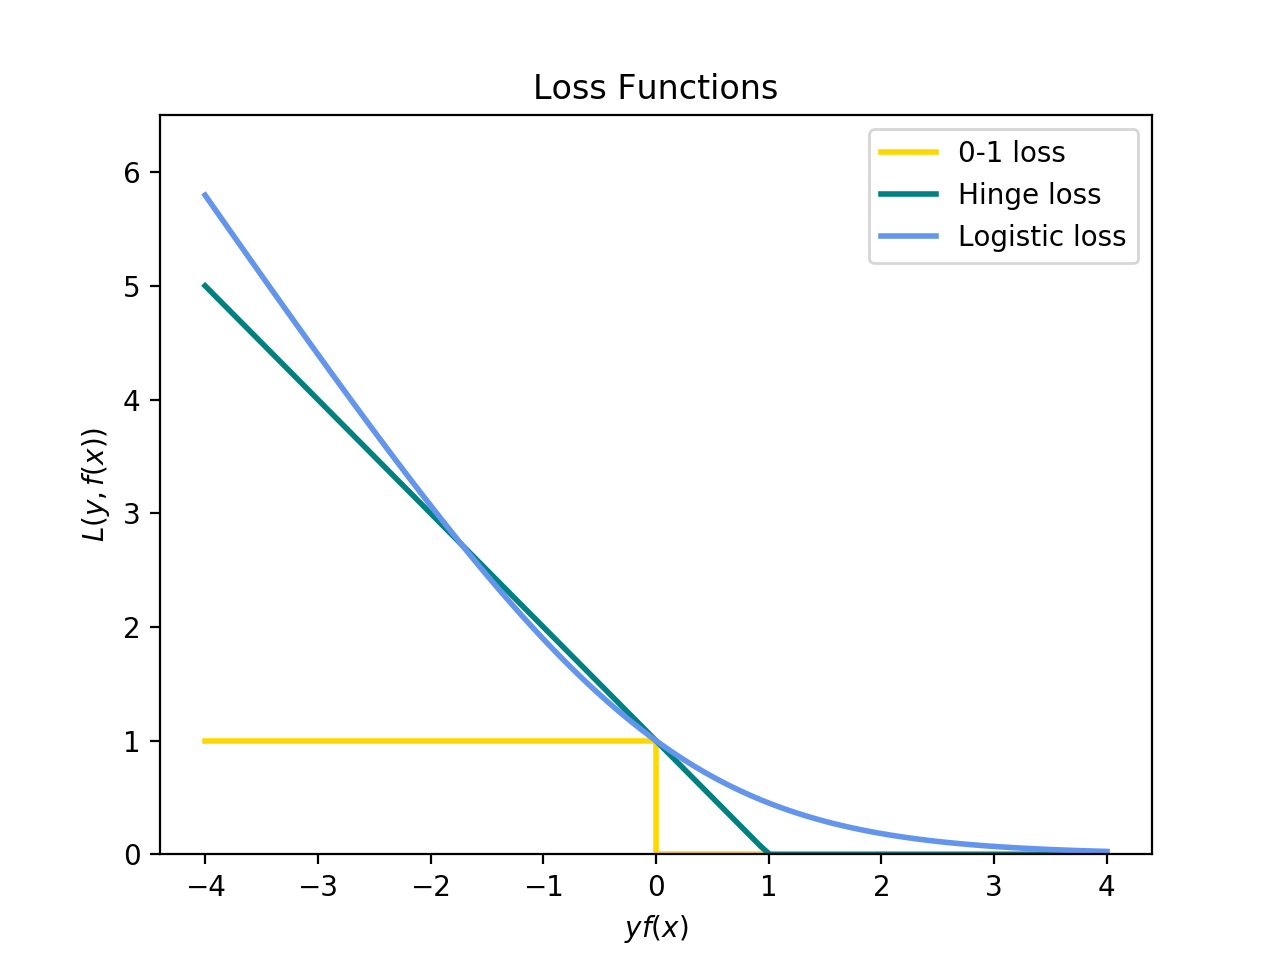
\includegraphics[0.8]{loss.png}
    \end{enumerate}  
    
    
    \item Prove that SPO loss is discontinuous and nonconvex.
    
    SPO loss: $\ell_{\mathrm{SPO}}(\hat{c}, c):=\max _{w \in W^{*}(\hat{c})}\left\{c^{T} w\right\}-z^{*}(c)$
    \begin{enumerate}
    
        \item Discontinuous
        
        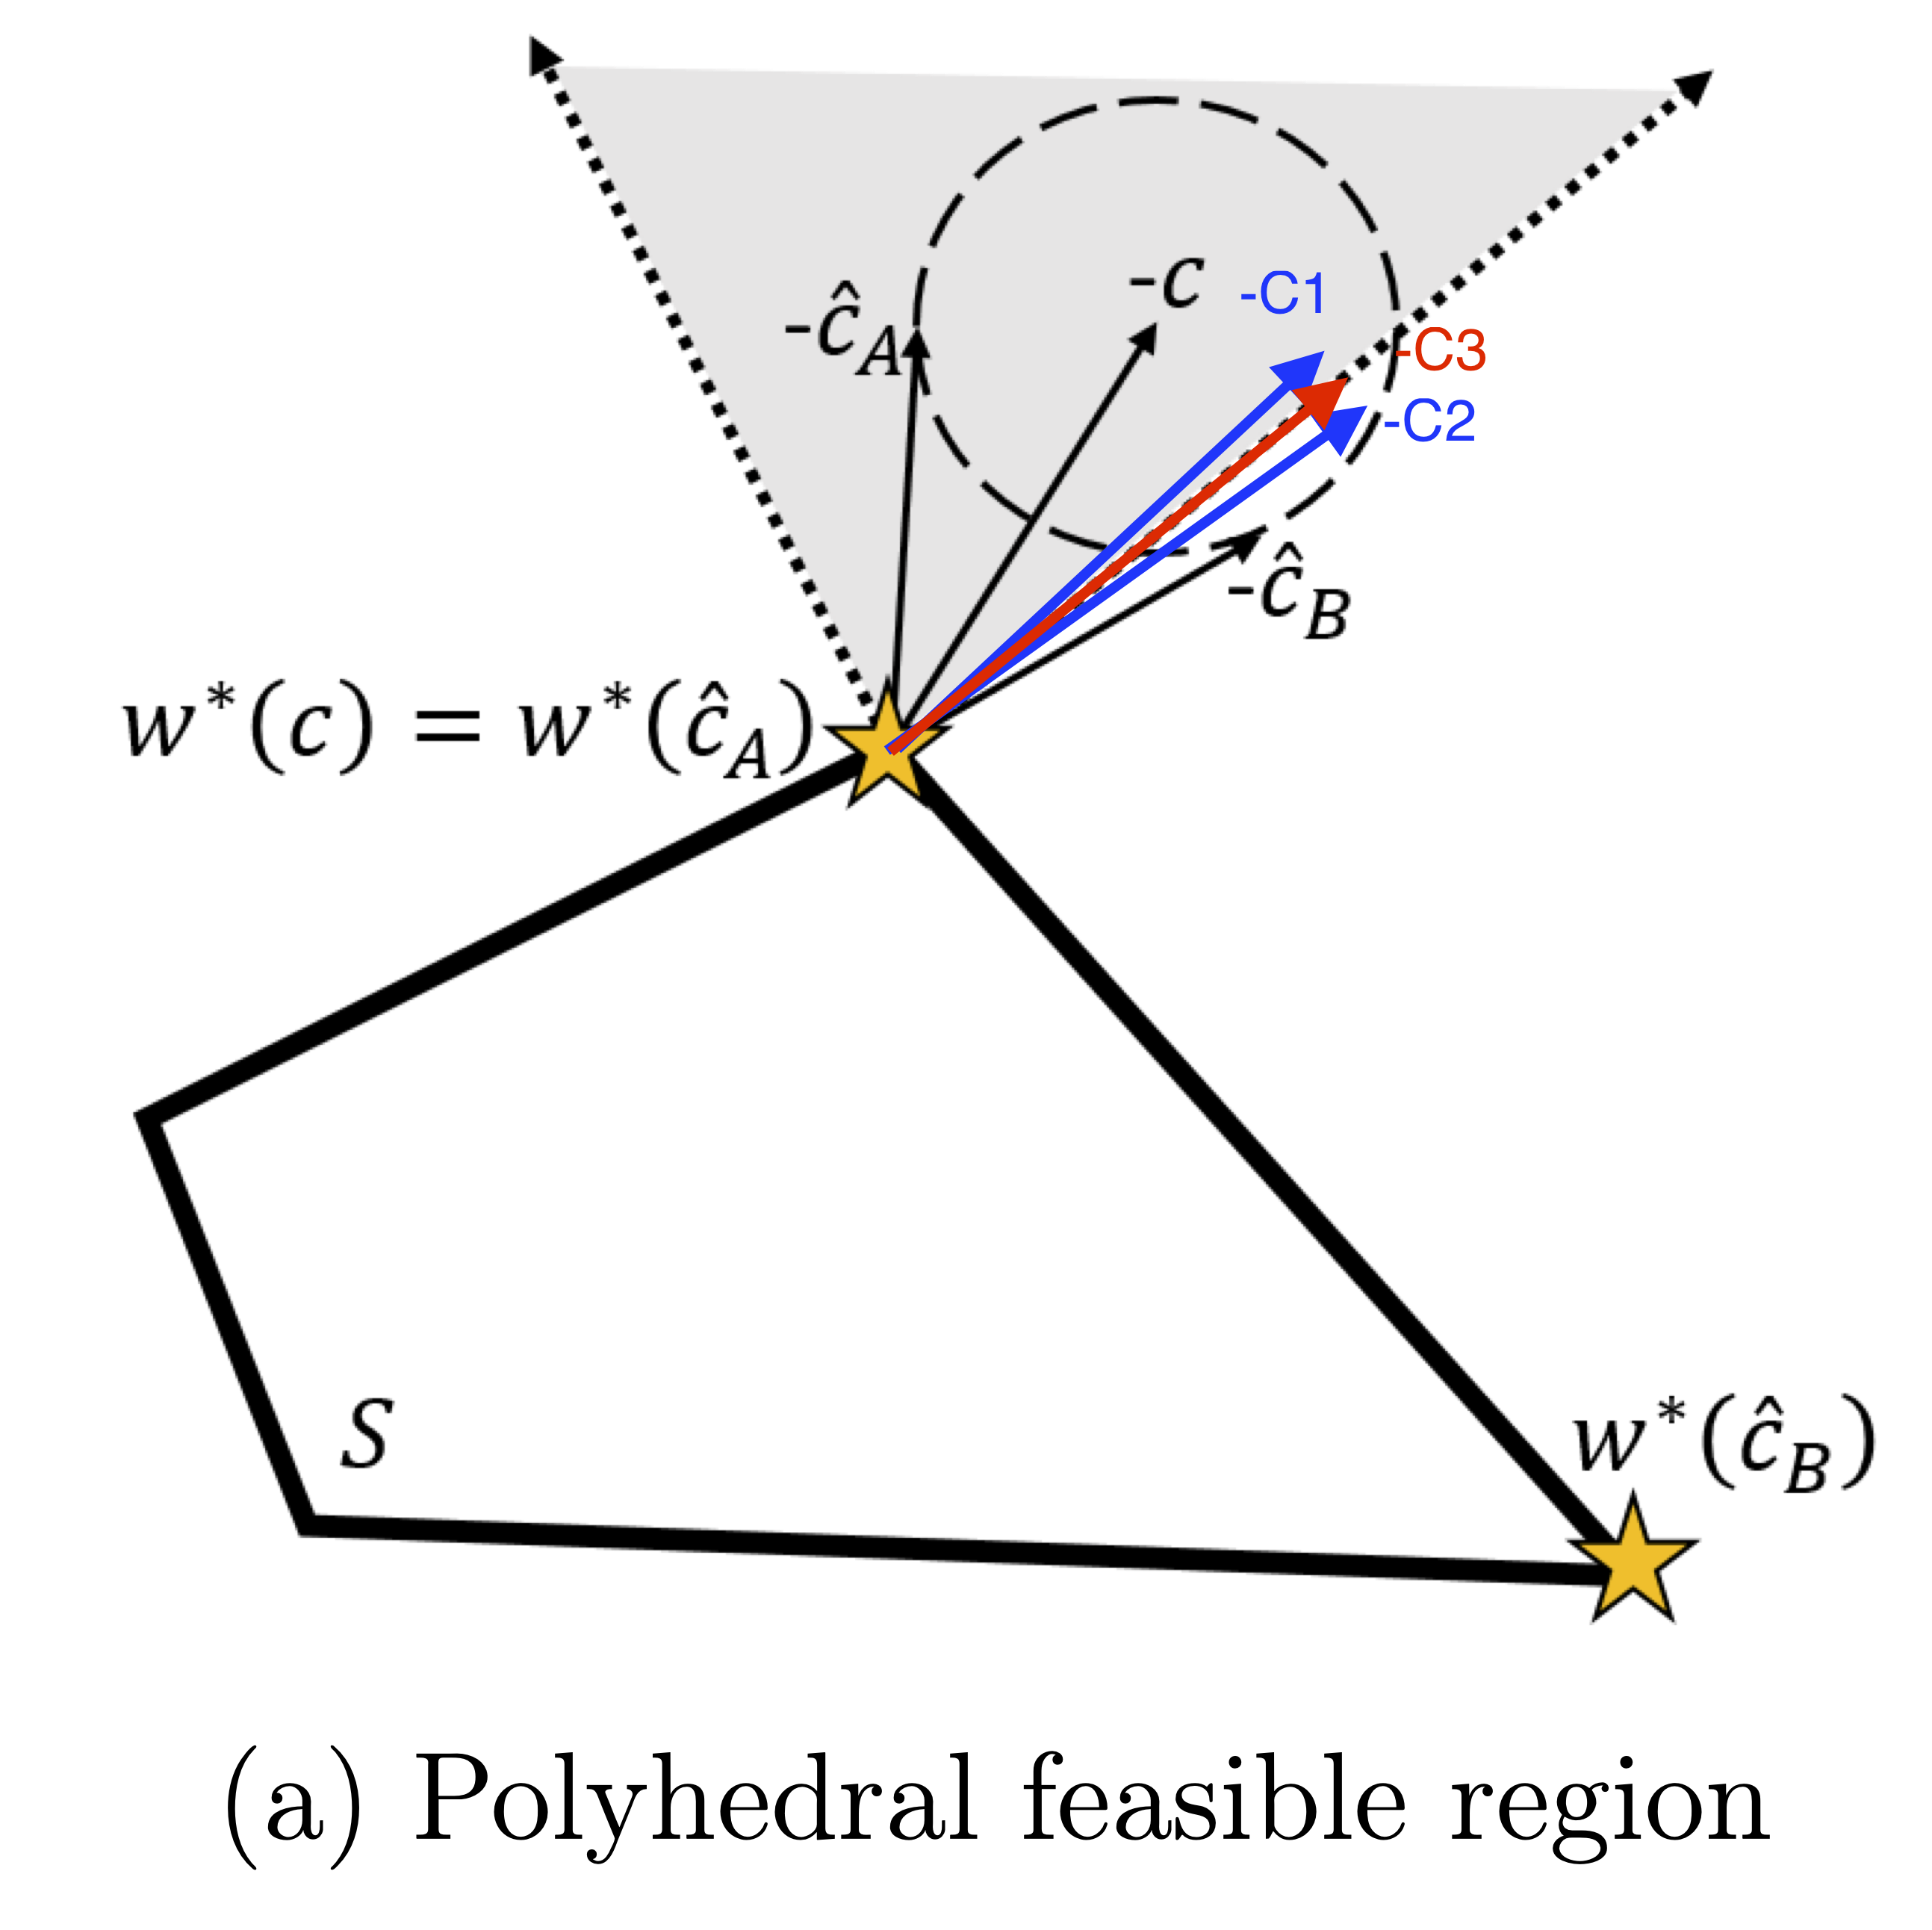
\includegraphics[width=0.5\textwidth]{discontinuous.png}
        
       Take the figure on page 10 as an example. $\hat{c_1}$ , $\hat{c_2}$ and $\hat{c_3}$ are three predicted values of $c$. $\hat{c_3}$ lies on the dotted line, and $\hat{c_1}$ , $\hat{c_2}$ lie in different sides of the line. They result in different decisions, $w^*(\hat{c_1})=w^*(\hat{c_3})=w^*(\hat{c_A})$, $w^*(\hat{c_2})=w^*(\hat{c_B})$. We consider the limit of $\ell_{\mathrm{SPO}}(\hat{c}, c)$ at point $\hat{c_3}$. When we approach $\hat{c_3}$ from $\hat{c_1}$, the limit is $c^{T} w^*(\hat{c_A})-z^{*}(c)$, but when we approach $\hat{c_3}$ from $\hat{c_2}$, the limit is $c^{T} w^*(\hat{c_B})-z^{*}(c)$. The two limits are different, so the SPO loss is discontinuous at $\hat{c_3}$. 
        
        
        \item Nonconvex
        
        I would like to show that 0-1 loss for binary classification is non-convex.
        \\0-1 loss function L is:
        \[L(x)=\left\{\begin{array}{ll}
0, & \text { if } x \geq 0 \\
1, & \text { if } x<0
\end{array}\right.\]
        If L is convex, for $x_1, x_2\in R$ and $\lambda \in[0,1]$, then:
        \[L\left(\lambda x_{1}+(1-\lambda) x_{2}\right) \leq \lambda L\left(x_{1}\right)+(1-\lambda) L\left(x_{2}\right)\]
        Here is a counterexample, if $\left(x_{1}, x_{2}, \lambda\right)=(-1,1 / 2,1 / 2)$,
        \[\begin{aligned}
L\left(\lambda x_{1}+(1-\lambda) x_{2}\right) &=L(-1 / 4)=1 \\
L\left(x_{1}\right) &=1 \\
L\left(x_{2}\right) &=0
\end{aligned}\]
        So, $L\left(\lambda x_{1}+(1-\lambda) x_{2}\right) \leq \lambda L\left(x_{1}\right)+(1-\lambda) L\left(x_{2}\right)$ does not hold. So, L is not convex.
    \end{enumerate}
    
\end{enumerate}


\end{document}
